% Part (b): the resulting weight-magnitude distribution shift.
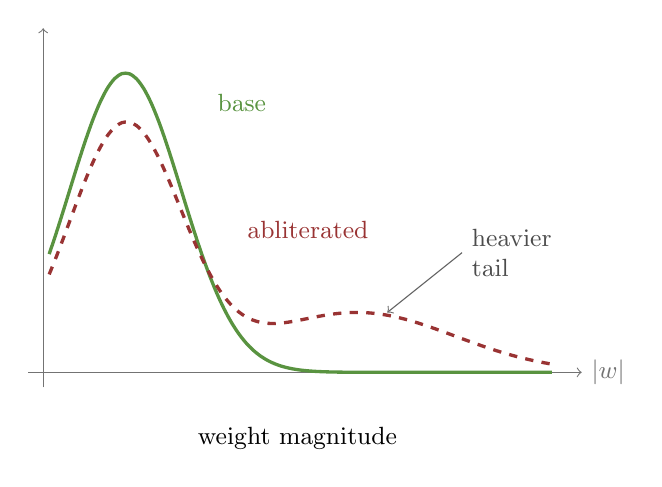
\begin{tikzpicture}[font=\small, x=1.9mm, y=1.9mm]
  \draw[->, black!55] (-1,0) -- (36,0) node[right, font=\small] {$|w|$};
  \draw[->, black!55] (0,-1) -- (0,23);
  \draw[OliveGreen!80, very thick, smooth, samples=70, domain=0.4:34]
    plot (\x, {20*exp(-((\x-5.5)^2)/28)});
  \draw[Maroon!80, very thick, dashed, smooth, samples=70, domain=0.4:34]
    plot (\x, {16.5*exp(-((\x-5.5)^2)/28) + 4.0*exp(-((\x-21)^2)/85)});
  \node[font=\small, text=OliveGreen!80, anchor=west] at (11,18)  {base};
  \node[font=\small, text=Maroon!80,   anchor=west] at (13,9.5) {abliterated};
  \draw[<-, black!60] (23,4.0) -- (28,8.0)
    node[anchor=west, font=\small, text=black!70, align=left] {heavier\\tail};
  \node[font=\small, anchor=north] at (17,-3) {weight magnitude};
\end{tikzpicture}
